% LaTeX Template for short student reports.
% Citations should be in bibtex format and go in references.bib
\documentclass[a4paper, 11pt]{article}
\usepackage[top=3cm, bottom=3cm, left = 2.5cm, right = 3cm]{geometry}
\usepackage[english]{babel} 
\geometry{a4paper} 
\usepackage[utf8]{inputenc}
\usepackage{textcomp}
\usepackage{graphicx} 
\usepackage{amsmath,amssymb} 
\usepackage{mathtools} 
\usepackage{bm}  
\usepackage[hidelinks]{hyperref} 
\usepackage{float}

\usepackage{setspace}
\onehalfspacing

\usepackage{pgfplots}
\pgfplotsset{width=10cm,compat=1.9}

\setlength{\parindent}{0cm}
%\hypersetup{linkcolor=black,citecolor=black,filecolor=black,urlcolor=black} % black links, for printed output
\usepackage{memhfixc} 
\usepackage{pdfsync}  
\usepackage{fancyhdr}
\pagestyle{fancy}

\usepackage[compact]{titlesec}  
\titlespacing*{\section}{0pt}{10ex plus 1ex minus .2ex}{4.3ex plus .2ex}

\usepackage[backend=biber, maxbibnames=99]{biblatex}


\usepackage{amsthm}


\newtheorem*{example*}{Example}




\addbibresource{references.bib}

\title{Runtime analysis of the Java implementation of the CYK-algorithm}
\author{Pina Kolling \\ piko0011@student.umu.se}
%\date{}


\newcommand{\dq}{"}






%---------------------------------------------------------------------%

%---------------------------------------------------------------------%






\begin{document}


\begin{titlepage}
	\centering
	{\scshape\LARGE Ume\r{a} University \par}
	Efficient Algorithms \par
	\vspace{1cm}
	{\scshape\Large Assignment Step 2 \par }
	\vspace{1.5cm}
	{\huge\bfseries  Runtime analysis of the Java implementation of the CYK-algorithm \par}
	\vspace{2cm}
	{\Large\itshape Pina Kolling\par}
	\vfill

% Bottom of the page
	{\large \today\par}
\end{titlepage}








%---------------------------------------------------------------------%







\setcounter{page}{1}


\newpage
\fancyhead[LO]{\empty}
{
  \hypersetup{linkcolor=black}
  \tableofcontents
}




\newpage





%---------------------------------------------------------------------%








\section{Introduction}

Parsing in Computer Science is the process of analysing a string of characters to examine if the string is built according to the rules of a formal grammar. 

A formal grammar describes how to form strings with correct syntax from a language's alphabet (section \ref{formalgrammar} and \ref{formallanguage}).
To examine if such a string follows the rules of a grammar the \textit{Cocke-Younger-Kasami}-algorithm (short: \textit{CYK}) can be used. This algorithm is described in section \ref{cyk}. To use the \textit{CYK}-algorithm the grammar needs to be in a specific format, that is called \textit{Chomsky-Normal-Form} (\textit{CNF}), which is explained in section \ref{cnf}. \cite{CYK_name, CYK1}


The task for this assignment was to code three different parsing methods to execute the \textit{CYK}-algorithm in \textit{Java}. The different parsing methods will be described and presented as pseudo code in section \ref{systemdesign}.
For the implementation three different classes were implemented: \texttt{main.java, grammar.java} and \texttt{parser.java}. The \texttt{main}-class calls the methods and the \texttt{grammar}-class parses the input grammer ans string into a format that then can be processed in the \texttt{parser}-class.
The function and implementation will be former described in section \ref{systemdesign}.




\pagebreak






%---------------------------------------------------------------------%








\section{Background}

In this section background information on formal languages (section \ref{formallanguage}), formal grammars (section \ref{formalgrammar}), Chomsky-Normal-Form (section \ref{cnf}), CYK-algorithm (section \ref{cyk}) and dynmaic programming (section \ref{dp}) will be presented. 

%---------------------------------------------------------------------%

\subsection{Formal language}
\label{formallanguage}
Formal languages are abstract languages which define the syntax of the words that get accepted by that language. It consits of a set of words that get accepted by the language and a set of symbols that is called alphabet and contains the characters of the words. Those characters are calles nonterminal symbols. \cite{CNF, language}

\begin{example*}[Formal language]
\footnote{The following examples show the \textit{Well-Balanced Parantheses} example from the assignment task sheet with the alphabet $\{a, b\}$ instead of $\{(, )\}$. }
\\
The language accepts words that contain the same number of $a$s and $b$s, while the a has to be left of the b. 
The alphabet $\Sigma$ of this language looks like this:
\begin{align*}
\Sigma = \{ a, b\}
\end{align*}
The language definition $L$ is the following one:
\begin{align*}
L = \{ (a^{n}b^{n})^m \} \text{ with } n, m \in \mathbb{N}
\end{align*}

\end{example*}



%---------------------------------------------------------------------%

\subsection{Formal grammar}
\label{formalgrammar}
A formal grammar describes how to form strings with correct syntax from a language's alphabet. A grammar does not describe the meaning of the strings or any semantics — only their syntax is defined. The grammar is a set of rules which define which words are accepted by a formal language. Those rules consist of terminal and nonterminal symbols. The terminalsymbols are the characters of the alphabet of the language and the nonterminalsymbols are used to build the rules of the language -- they get replaced by terminalsymbols. \cite{CNF, language} 

\begin{example*}[Formal grammar]
The example grammar for the previous example language is the following:
\begin{center}
\texttt{S $\rightarrow$ SS $\mid$  aSb $\mid$ ab}
\end{center}
\end{example*}

%---------------------------------------------------------------------%

\subsection{Chomsky-Normal-Form}
\label{cnf}
The \textit{Chomsky-Normal-Form} (short: \textit{CNF}) is a grammar which is formated in a specific way. If the startsymbol (nonterminal symbol) is not generating the empty word (\textit{\texttt{S $\rightarrow \epsilon$}}) it either generates two nonterminal symbols or one terminal symbol for the grammar to be in \textit{CNF}.
\cite{CNF}

\begin{example*}[Chomsky-Normal-Form]
To change the previous example into CNF the rules have to be split up:
\begin{align*}
\texttt{S} & \rightarrow \texttt{SS} \mid  \texttt{LA} \mid \texttt{LR} \\
\texttt{A} & \rightarrow \texttt{SR} \\
\texttt{L} & \rightarrow a \\
\texttt{R} & \rightarrow b
\end{align*}
\end{example*}


%---------------------------------------------------------------------%

\subsection{CYK-algorithm}
\label{cyk}
\textit{Cocke-Younger-Kasami}-algorithm (short: \textit{CYK}) takes a grammar in \textit{CNF} and a word as an input. It then examines if the word follows the rules of the grammar. \cite{CYK1}

\begin{example*}[Chomsky-Normal-Form]
The following table shows the CYK-algorithm with the previous grammar example and the input word $aaabbb$. \cite{cyk_online_alg}
\begin{figure}[H]
\begin{center}
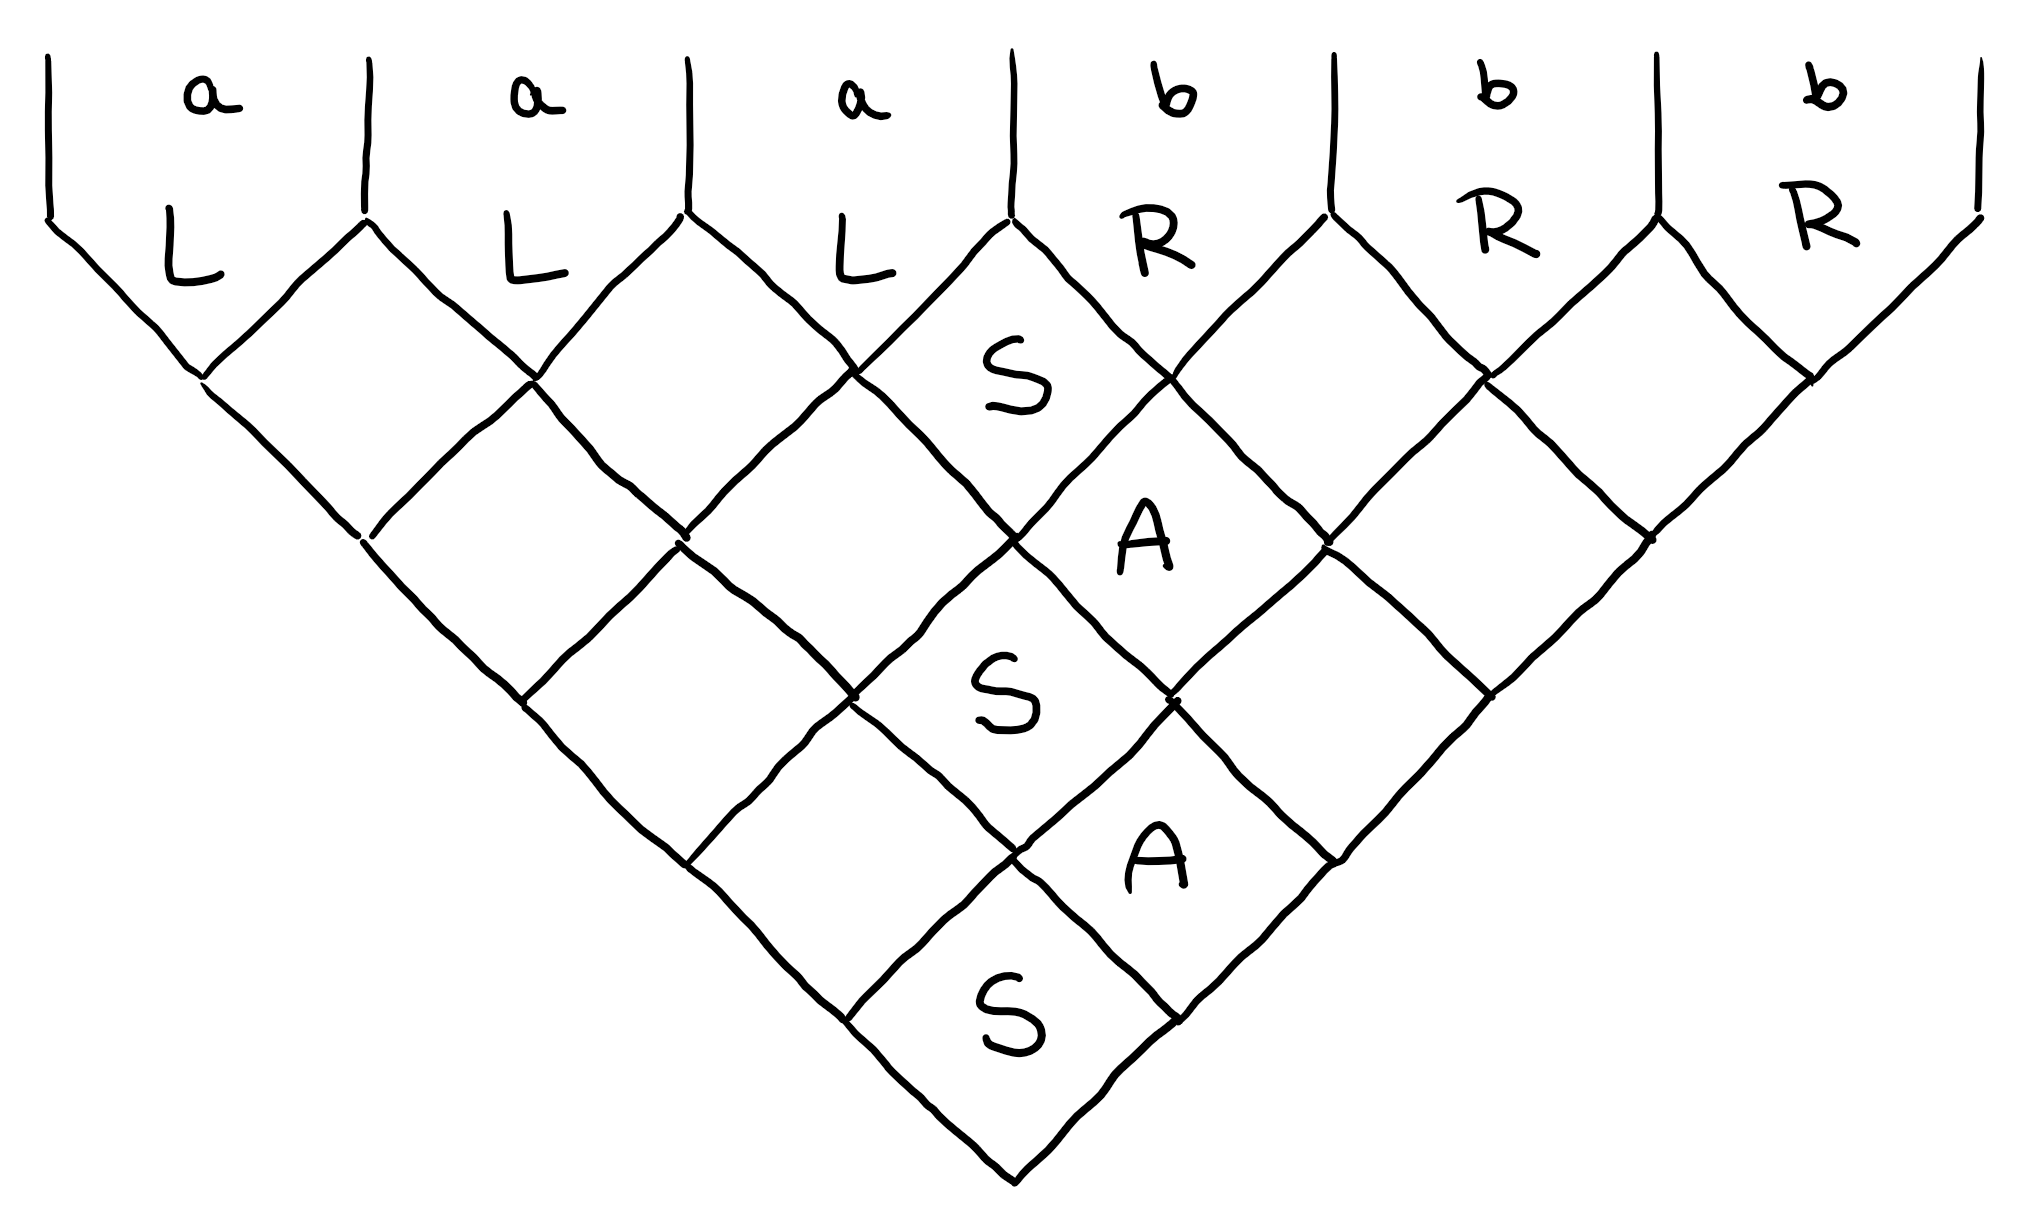
\includegraphics[scale=0.3]{images/cyk_table.png}
\end{center}
\caption{CYK-algorithm table for the word $aaabbb$}
\end{figure}
The word is accepted by the grammar rules, because the intiating nonterminal symbol \textit{\texttt{S}} can be filled into the lowest field.
\end{example*}

%---------------------------------------------------------------------%

\subsection{Dynamic programming}
\label{dp}

The technique of dynamic programming can be used to solve problems, which can be devided into smaller subproblems. The solutions of the subproblems are saved (for example in a multi-dimensional array) and referenced later. \cite{DP}


%---------------------------------------------------------------------%



\pagebreak





%---------------------------------------------------------------------%








\section{System Design}
\label{systemdesign}

The implementation was done in Java and three different classes were implemented: \texttt{main.java} (described in section \ref{main}), \texttt{grammar.java} (described in section \ref{grammar}) and \texttt{parser.java} (described in section \ref{parser}). The \texttt{main}-class calls the methods and the \texttt{grammar}-class parses the input grammer ans string into a format that then can be processed in the \texttt{parser}-class.


%---------------------------------------------------------------------%



\subsection{Main}
\label{main}

The \texttt{main}-class takes the input grammar and word and parses them into \texttt{String[]} and \texttt{String}. The arguments have to follow the following rules:
\begin{itemize}
\item The Grammar needs to be in \textit{CNF}.
\item The first rule begins with the start symbol of the grammar.
\item The rules are put in wothout arrows, one rule body is represented by one string, beginning with the rule head.
\item The last argument is the input word.
\end{itemize}
Input example (\textit{Well-Balanced-Parantheses}):\\
  \texttt{java Main \dq SSS\dq \ \dq SLA\dq \ \dq SLR\dq \ \dq ASR\dq \ \dq L(\dq \ \dq R)\dq\  \dq (())\dq}
\\ 
for the grammar \texttt{S $\rightarrow$ SS | LA | LR, A $\rightarrow$ SR, L $\rightarrow$ (, R $\rightarrow$ )} and the input word \texttt{(())}. \\


%---------------------------------------------------------------------%
%---------------------------------------------------------------------%

\subsection{Grammar}
\label{grammar}



\begin{minipage}{0.6\textwidth}
\vspace*{-2em}

The \texttt{grammar}-class assigns the nonterminal symbols to integers and builds arrays with them. The start symbol for example is then assigned with the integer zero and the bodies of that rule are at the index zero of an two-dimensional array. One array that only contains nonterminal symbols is build, one array that contains terminal and nonterminal symbold and one array that represents the integers that represent each nonterminal symbol is built.

For the input \texttt{java Main \dq SSS\dq \ \dq SLA\dq \ \dq SLR\dq \ \dq ASR\dq \ \dq L(\dq \ \dq R)\dq\  \dq (())\dq} the two-dimensional arrays shown on the screenshot on the right side are built.

(Right now the arrays still have the type \texttt{String[][]}, that will be changed later to \texttt{int[][][]} to minimize the access time in the parsing methods.)


\end{minipage}\begin{minipage}{0.1\textwidth}
\ 
\end{minipage}\begin{minipage}{0.3\textwidth}
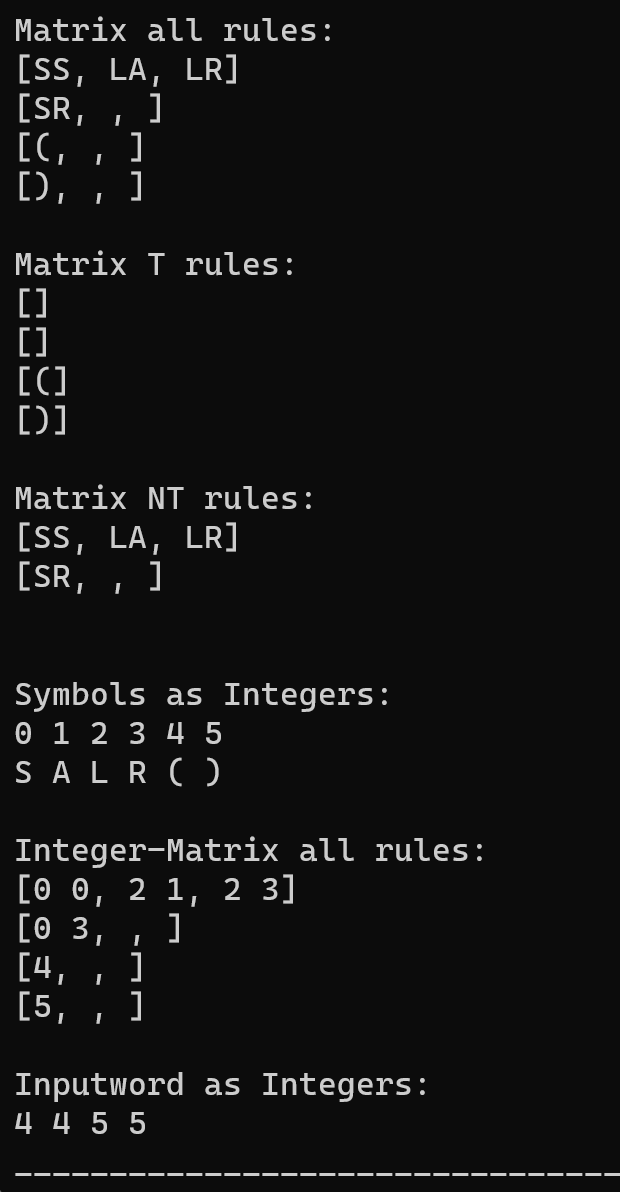
\includegraphics[scale=0.6]{images/terminal_1.png}
\end{minipage}


%---------------------------------------------------------------------%
%---------------------------------------------------------------------%

\subsection{Parser}
\label{parser}

%---------------------------------------------------------------------%

\subsubsection{Naive}
\label{naive}

%---------------------------------------------------------------------%

\subsubsection{Bottom-Up}
\label{bottomup}

%---------------------------------------------------------------------%

\subsubsection{Top-Down}
\label{topdown}

%---------------------------------------------------------------------%

\pagebreak






%---------------------------------------------------------------------%







\section{Evaluation}

We did some experiments \ldots

\pagebreak





%---------------------------------------------------------------------%








\section{Conclusions and Future Work}

From our experiments we can conclude that \ldots

\newpage





%---------------------------------------------------------------------%








\appendix

\section{How to use the code?}

The code can be run in the terminal and input is expected as Strings in quotation marks. The grammar needs to be in CNF. The first rule begins with the startsymbol of the grammar. \\ \\
First: Rules without arrows (one rule as one String) \\
Last: The last argument is the input word
\\ 

Input example (\textit{Well-Balanced-Parantheses}):\\
  \texttt{java Main \dq SSS\dq \ \dq SLA\dq \ \dq SLR\dq \ \dq ASR\dq \ \dq L(\dq \ \dq R)\dq\  \dq (())\dq}
\\ 
for the grammar \texttt{S $\rightarrow$ SS | LA | LR, A $\rightarrow$ SR, L $\rightarrow$ (, R $\rightarrow$ )} and the input word \texttt{(())}.
\\ \\
Output example: \\
The first part of the output shows the arrays, which get generated in the \texttt{Grammar.java} class.  \\ \\
\begin{minipage}{0.6\textwidth}
\vspace*{-2em}
The first array contains all rules. \\ \\ \\

The second array contains only the terminal rules. \\ \\

The third array contains only the nonterminal rules. \\

Then it is shown which nonterminal symbols are represented by which integers. Later the nonterminal symbols can be referred to with those integers. \\ 

After this the mentioned arrays are shown again but the nonterminal symbols got replaced with the according integers.

\end{minipage}\begin{minipage}{0.2\textwidth}
\ 
\end{minipage}\begin{minipage}{0.3\textwidth}
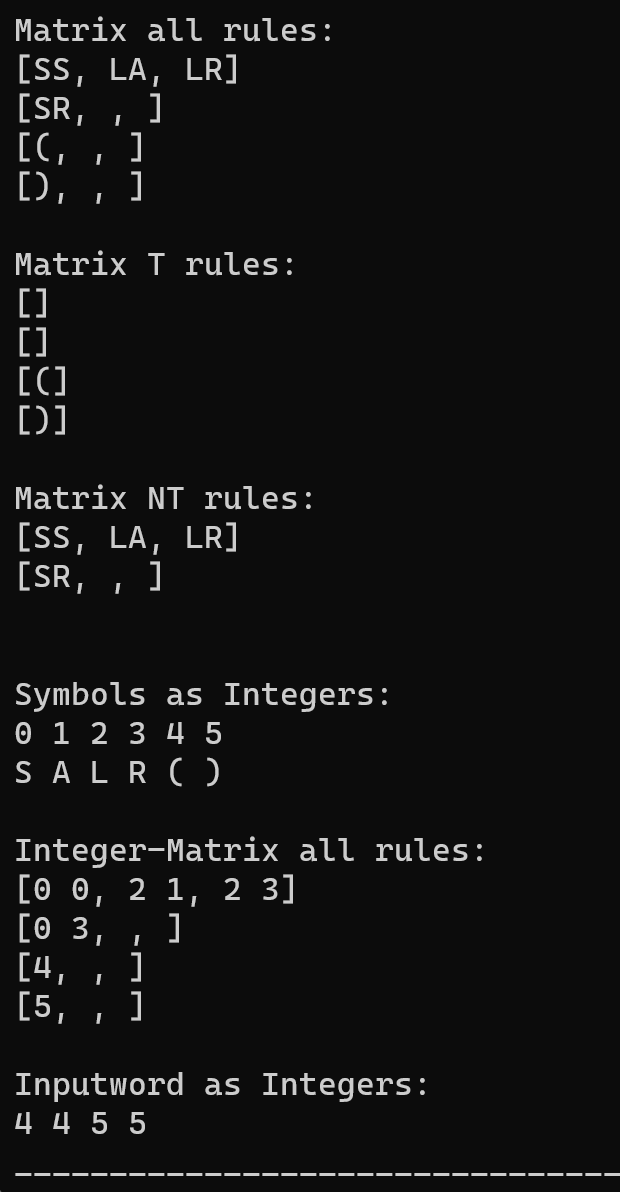
\includegraphics[scale=0.7]{images/terminal_1.png}
\end{minipage}

\begin{minipage}{0.4\textwidth}
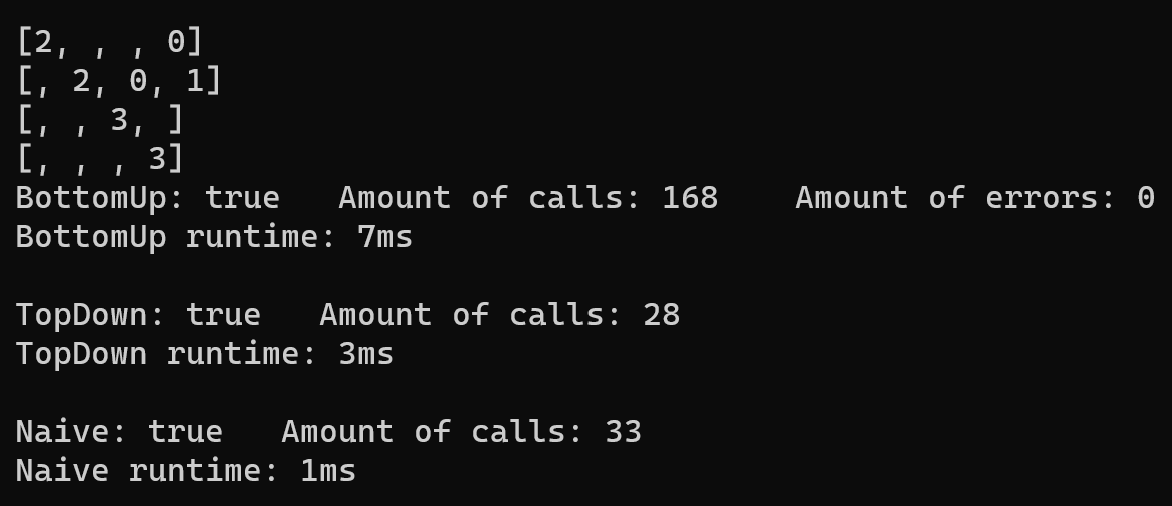
\includegraphics[scale=0.6]{images/terminal_2.png}
\end{minipage}\begin{minipage}{0.6\textwidth}
Then the results, counter and runtime in $ms$ is shown for each parsing method. \\
For the \texttt{BottomUp} method is the CYK algorithm table printed.
\end{minipage}









%---------------------------------------------------------------------%







\fancyhead[LO]{\empty}




\newpage
\phantomsection
\addcontentsline{toc}{section}{\bibname}
%\begin{spacing}{1.3}
\printbibliography
%\end{spacing}



\end{document}